%
% f.tex -- Wavelet spectrum
%
% (c) 2019 Prof Dr Andreas Müller, Hochschule Rapperswil
%
\documentclass[tikz]{standalone}
\usepackage{amsmath}
\usepackage{times}
\usepackage{txfonts}
\usepackage{pgfplots}
\usepackage{csvsimple}
\usetikzlibrary{arrows,intersections,math}
\begin{document}

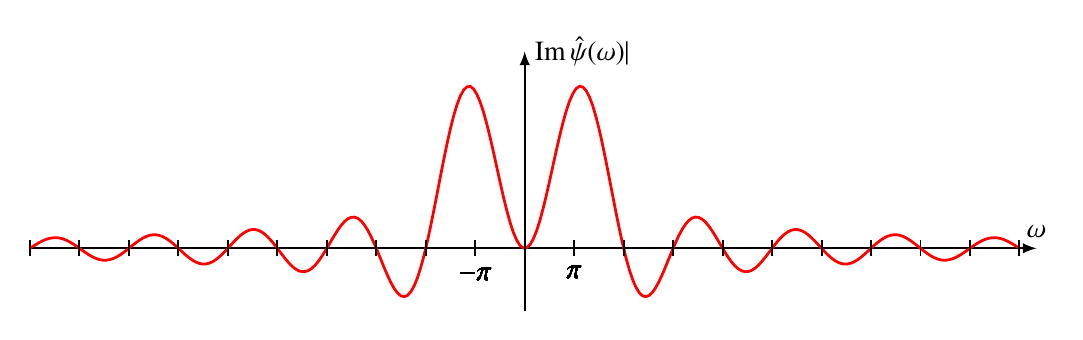
\begin{tikzpicture}[>=latex]
\def\perioden{5}
\draw[->,line width=0.7pt] (-6.3,0)--(6.5,0) coordinate[label={$\omega$}];
\draw[->,line width=0.7pt] (0,-0.8)--(0,2.5) coordinate[label={right:$\operatorname{Im}\hat{\psi}(\omega)|$}];
\draw[color=red,line width=1pt] plot[domain=-{\perioden*360+1}:{\perioden*360+1},samples=300]
	({\x*3.1415/(\perioden*180)},{5*(sqrt(2)/sqrt(3.14159))*sin(\x)*(\x/180)/(3.14159*(1-(\x/180)*(\x/180)))});
\foreach \x in {-10,...,10}{
	\draw[line width=0.7pt] ({\x*3.1415/\perioden},-0.1)--({\x*3.1415/\perioden},0.1);
	\node at ({3.14159/\perioden},-0.1) [below] {$\pi$};
	\node at ({-3.14159/\perioden},-0.1) [below] {$-\pi$};
}
\end{tikzpicture}
\end{document}
